\section{The Advantage Of Traces}
\label{sec:advantage-traces}
In this section we present a qualitative evaluation of the witnesses and
traces that \toolname produces.

\begin{figure*}[ht]
\centering
\begin{minipage}{0.49\linewidth}
\centering
\begin{code}
let rec sqsum xs = match xs with
  | [] -> 0
  | h::t -> (sqsum t) @ (h * h)
\end{code}
\begin{verbatim}
File "prog3151.ml", line 7, characters 12-21:
Error: This expression has type
         int
       but an expression was expected of type
         'a list
\end{verbatim}
\end{minipage}
\begin{minipage}{0.49\linewidth}
\centering
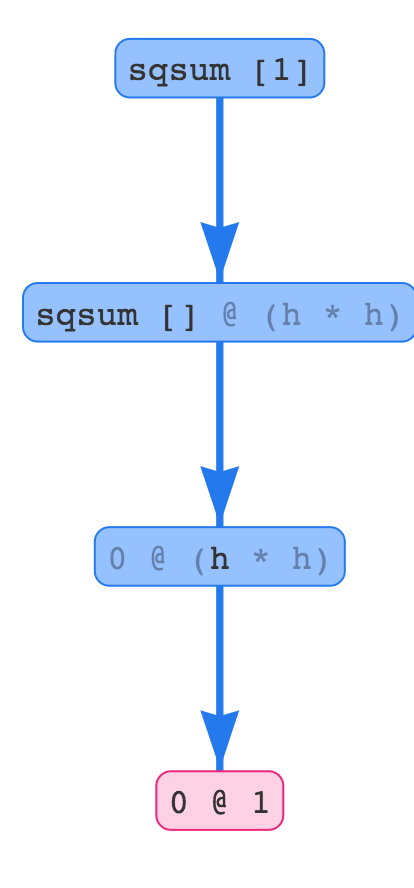
\includegraphics[height=200px]{sqsum.png}
\end{minipage}
\caption{caption}
\label{fig:traces}
\end{figure*}

\begin{figure*}[ht]
\centering
\begin{minipage}{0.49\linewidth}
\centering
\begin{code}
let rec sumList xs = match xs with
  | []    -> []
  | y::ys -> y + sumList ys
\end{code}
\begin{verbatim}
File "sumlist.ml", line 5, characters 17-27:
Error: This expression has type
         'a list
       but an expression was expected of type
         int
\end{verbatim}
\end{minipage}
\begin{minipage}{0.49\linewidth}
\centering
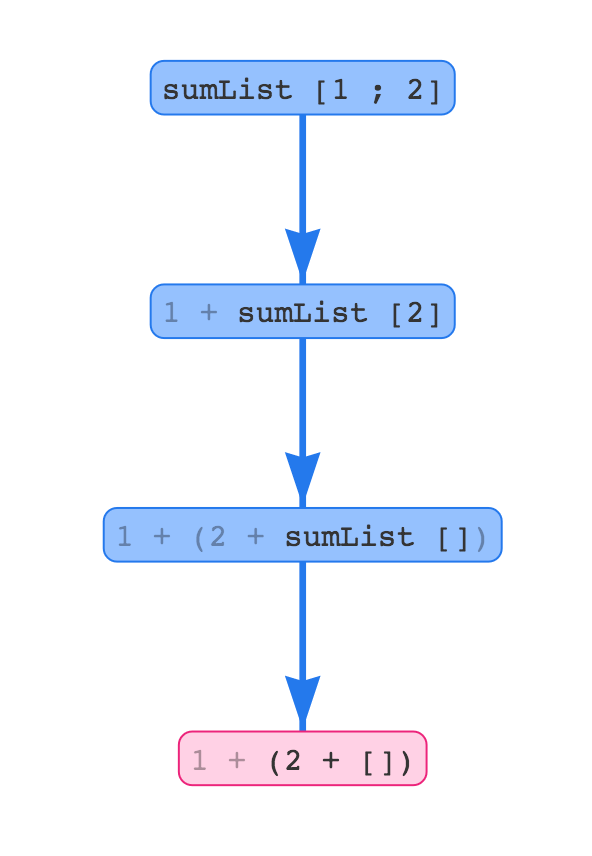
\includegraphics[height=200px]{sumlist.png}
\end{minipage}
\caption{caption}
\label{fig:traces}
\end{figure*}

\begin{figure*}[ht]
\centering
\begin{minipage}{0.49\linewidth}
\centering
\begin{code}
let append xs ys = match xs with
  | []   -> ys
  | h::t -> h :: t :: ys
\end{code}
\begin{verbatim}
File "prog0164.ml", line 7, characters 17-18:
Error: This expression has type
         'a list
       but an expression was expected of type
         'a
       The type variable 'a occurs inside 'a list
\end{verbatim}
\end{minipage}
\begin{minipage}{0.49\linewidth}
\centering
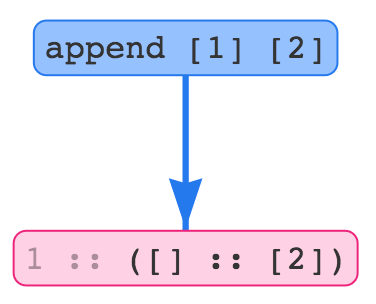
\includegraphics[height=100px]{append.png}
\end{minipage}
\caption{caption}
\label{fig:traces}
\end{figure*}

\begin{figure*}[ht]
\centering
\begin{minipage}{0.49\linewidth}
\centering
\begin{code}
let rec wwhile (f,b) =
  match f with
  | (z, false) -> z
  | (z, true)  -> wwhile (f, z)

let f x =
  let xx = x * x in
  (xx, (xx < 100))

let _ = wwhile (f, 2)
\end{code}
\begin{verbatim}
File "prog0358.ml", line 19, characters 16-17:
Error: This expression has type
         int -> int * bool
       but an expression was expected of type
         'a * bool
\end{verbatim}
\end{minipage}
\begin{minipage}{0.49\linewidth}
\centering
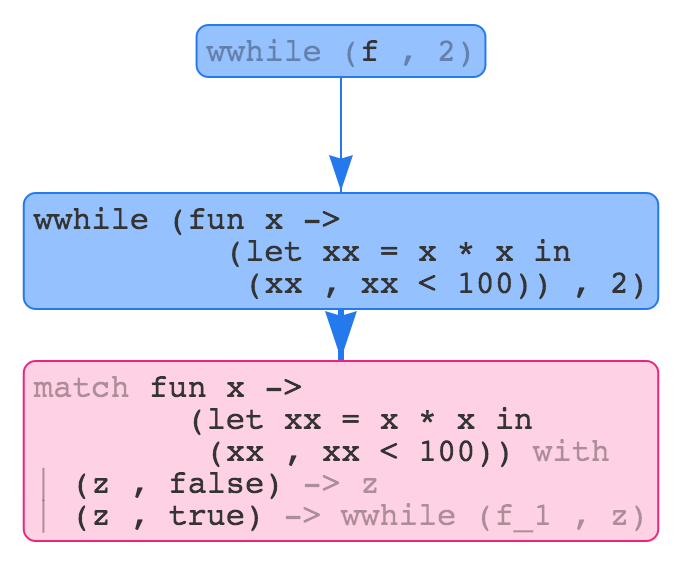
\includegraphics[height=150px]{wwhile.png}
\end{minipage}
\caption{caption}
\label{fig:traces}
\end{figure*}














%%% Local Variables:
%%% mode: latex
%%% TeX-master: "main"
%%% End:
